% arXiv categories: cs.AI (primary), cs.CL, cs.MA (secondary)
% arXiv identifier: [to be assigned]
\pdfoutput=1
\documentclass[11pt,letterpaper]{article}

% ============================================================
% PACKAGES
% ============================================================
\usepackage[utf8]{inputenc}
\usepackage[T1]{fontenc}
\usepackage{lmodern}
\usepackage[margin=1in,top=1.25in]{geometry}
\usepackage{graphicx}
\usepackage{booktabs}
\usepackage{array}
\usepackage{amsmath}
\usepackage{amssymb}
\usepackage{amsthm}
\usepackage{enumitem}
\usepackage{xcolor}
\usepackage{listings}
\usepackage{tikz}
\usepackage{algorithm}
\usepackage{algpseudocode}
\usepackage{float}
\usepackage{placeins}
\usepackage{natbib}
\usepackage{microtype}
\usepackage{fancyhdr}
\usetikzlibrary{shapes,arrows,positioning,fit,backgrounds,calc}

% hyperref loaded last
\usepackage[bookmarks=true,breaklinks=true]{hyperref}
\usepackage{url}

% ============================================================
% PAGE BREAK CONTROL
% ============================================================
\widowpenalty=10000
\clubpenalty=10000
\raggedbottom

% ============================================================
% THEOREM ENVIRONMENTS
% ============================================================
\newtheorem{definition}{Definition}[section]
\newtheorem{theorem}{Theorem}[section]
\newtheorem{lemma}[theorem]{Lemma}
\newtheorem{proposition}[theorem]{Proposition}

% ============================================================
% CUSTOM TITLE FORMATTING (NeurIPS-like)
% ============================================================
\makeatletter
\def\@maketitle{%
  \newpage
  \null
  \vskip 0.5em%
  {\centering
    \rule{\textwidth}{1.5pt}\\[0.4em]
    {\LARGE\bfseries \@title \par}%
    \vskip 0.4em%
    \rule{\textwidth}{0.4pt}\\[1.5em]
    \@author\par
  }%
  \vskip 1.5em}
\makeatother

% Abstract styling
\renewenvironment{abstract}{%
  \vskip 1em%
  \begin{center}%
    \bfseries Abstract%
  \end{center}%
  \begin{quotation}%
    \small\noindent
}{%
  \end{quotation}%
  \vskip 1em%
}

% Footer with page numbers
\pagestyle{fancy}
\fancyhf{}
\renewcommand{\headrulewidth}{0pt}
\fancyfoot[C]{\thepage}

% ============================================================
% STYLING
% ============================================================
\hypersetup{
    colorlinks=true,
    linkcolor=blue!70!black,
    urlcolor=blue!70!black,
    citecolor=blue!70!black,
    pdftitle={An Argument for Externalized Epistemics},
    pdfauthor={Aliasgar Khimani},
    pdfkeywords={agent memory, epistemology, belief revision, externalized state, multi-agent coordination}
}

\lstset{
    basicstyle=\ttfamily\small,
    breaklines=true,
    frame=single,
    backgroundcolor=\color{gray!10}
}

% ============================================================
% DOCUMENT
% ============================================================
\begin{document}

% ------------------------------------------------------------
% TITLE
% ------------------------------------------------------------
\title{An Argument for Externalized Epistemics\\[0.4em]{\large\normalfont Why agent memory requires epistemic architecture.}}

\author{
    \textbf{Aliasgar Khimani}\\
    \texttt{aliasgar.khimani@engrammic.ai}\\
    Engrammic
}

\date{}

\maketitle

% ------------------------------------------------------------
% ABSTRACT
% ------------------------------------------------------------
\begin{abstract}
Where should an AI agent's knowledge live? Three architectural options exist: in model weights (learned memory), in the context window (session-scoped), or in an external epistemic store (persistent, auditable). We argue that externalization is not merely convenient but \textit{architecturally required} for agents that must maintain coherent beliefs over time, coordinate with other agents, or submit to audit.

We present convergent evidence from six domains: (1) \textbf{information theory}, where neural network weights have a capacity ceiling of approximately 3.6 bits per parameter, insufficient for open-ended knowledge accumulation; (2) \textbf{optimization theory}, where catastrophic forgetting is geometric, not incidental, as new-task gradients implicitly attack old-task knowledge; (3) \textbf{interpretability}, where superposition and nonidentifiability make ``what does the model believe?'' an ill-posed question; (4) \textbf{distributed systems}, where multi-agent coordination requires shared substrate per CAP theorem and Byzantine fault tolerance theory; (5) \textbf{neuroscience}, where biological memory systems externalize episodic content to the hippocampus before slow neocortical consolidation; (6) \textbf{systems theory}, where the separation of compute and storage is a foundational design principle.

We formalize these constraints as the \textbf{Externalized Epistemics Thesis}: any system requiring durable, auditable, multi-agent-coherent beliefs must maintain epistemic state outside the models doing inference. We present Layered Epistemic Agent Protocol (LeAP) as an architecture satisfying these requirements, achieving 95\% contradiction detection and 87\% revision propagation versus 66\% and 12\% for in-context baselines. The framework extends to latent-space epistemology for JEPA-style world models.
\end{abstract}

% ------------------------------------------------------------
% 1. INTRODUCTION
% ------------------------------------------------------------
\section{Introduction}

The question of where knowledge should live in an AI system is typically treated as an engineering decision: weights for ``baked-in'' knowledge, retrieval for dynamic content, context for session state. This framing obscures a deeper architectural constraint.

Consider three failure modes in production agent systems:

\begin{enumerate}[noitemsep]
    \item \textbf{Hallucination laundering}: An agent stores a hallucinated fact, retrieves it next session, and treats it as ground truth. The mem0 production audit (Issue \#4573)\footnote{\url{https://github.com/mem0ai/mem0/issues/4573}} documents 97.8\% junk rate with 808 duplicate assertions of ``User prefers Vim'', a hallucination that multiplied through feedback loops.

    \item \textbf{Contradiction accumulation}: An agent learns ``API uses OAuth2'' on Monday and ``API uses API keys'' on Tuesday. Both persist indefinitely. mem0 Issue \#4896 (closed ``not planned'')\footnote{\url{https://github.com/mem0ai/mem0/issues/4896}} confirms the architecture cannot resolve semantic contradictions.

    \item \textbf{Coordination failure}: Multiple agents write to shared state, each maintaining its own version of truth. The MAST taxonomy~\cite{mast2025} finds 79\% of multi-agent failures are coordination errors.
\end{enumerate}

These are not implementation bugs but consequences of where knowledge lives: in-weights memory cannot be queried, corrected, or audited; per-agent learned state cannot achieve multi-agent consensus; session-scoped context cannot persist across sessions.

This paper argues that \textbf{externalized epistemics} (maintaining beliefs in a substrate external to the models doing inference) is architecturally required for any system with durability, auditability, or multi-agent coherence requirements.

\subsection{Common Workarounds}

Three responses to these failure modes are common in practice. Each fails for structural reasons.

\textbf{Database with timestamps.} ``Store facts in a database with timestamps for provenance.'' Timestamps provide history, not provenance. A database stores ``API uses OAuth2'' and ``API uses API keys'' with different timestamps but cannot determine which is current, whether they contradict, or whether downstream conclusions should be invalidated. The mem0 audit---808 duplicate ``User prefers Vim'' assertions---\textit{was} a database with timestamps. Logging everything is not the same as knowing why the system believes something.

\textbf{Ephemeral agent swarms.} ``Why long-running agents? Spin up targeted agents for each task.'' Swarms need externalized epistemics \textit{more}, not less. Coordination overhead scales with agent count. Knowledge must survive agent termination. Contradictions multiply across agents writing to shared state without coherence enforcement. Audit requires tracing across dead agents. Externalization is not for long-running agents specifically; it is for any system where knowledge crosses agent boundaries---which swarms do by definition.

\textbf{Orchestrator with sufficient context.} ``Use an orchestrator agent with a large context window; throw more tokens at it.'' This is the in-context baseline we evaluate in Section~\ref{sec:eval}: 66\% contradiction detection, 12\% revision propagation. Context is state, not structure---a blob of text with no epistemic types, no coherence invariants, no provenance chains. Context windows are finite; day 47, what was decided on day 3 is gone or garbled. Cost scales with memory size at inference prices. The orchestrator is a single point of failure with no persistence and no recovery.

\textbf{The scaling assumption.} These workarounds share an assumption: that architectural limits can be scaled around. Larger context windows. More agents. Cheaper inference. History suggests otherwise: efficiency gains enable increased usage rather than reducing total cost~\cite{jevons1865}. Weight capacity is bounded (Section~\ref{sec:thesis}). Context windows compress. Coordination overhead grows superlinearly with agent count.

Externalized epistemics is not an optimization but an acknowledgment: durable knowledge requires infrastructure, not larger inference budgets. The question is not ``how much can we scale?'' but ``what architecture respects the constraints?''

\subsection{Contributions}

\begin{enumerate}[noitemsep]
    \item \textbf{The Externalized Epistemics Thesis}: A formal argument, grounded in information theory, optimization theory, interpretability research, distributed systems, neuroscience, and systems theory, that epistemic state must be external to inference.

    \item \textbf{Layered Epistemic Agent Protocol (LeAP)}: A four-layer architecture implementing externalized epistemics with write-time coherence enforcement and AGM-compliant belief revision.

    \item \textbf{Empirical validation}: 95\% contradiction detection, 87\% revision propagation on 500 annotated coding-agent sessions.

    \item \textbf{Extension to world models}: Analysis of how externalized epistemics applies to JEPA-style latent-space architectures.
\end{enumerate}

The remainder of the paper is organized as follows. Section~\ref{sec:thesis} presents the Externalized Epistemics Thesis with evidence from six domains. Section~\ref{sec:leap} describes the LeAP architecture. Section~\ref{sec:eval} evaluates the system. Section~\ref{sec:extensions} discusses extensions to world models and multi-agent settings.

% ------------------------------------------------------------
% 2. THE EXTERNALIZED EPISTEMICS THESIS
% ------------------------------------------------------------
\section{The Externalized Epistemics Thesis}
\label{sec:thesis}

A system exhibits externalized epistemics when its belief state is maintained in a substrate that is (1) external to weights, (2) external to any single agent, (3) queryable, (4) correctable without retraining, and (5) auditable via provenance chains.

The thesis: any system requiring durable, auditable, multi-agent-coherent beliefs must externalize epistemic state. Evidence from six domains supports this.

\subsection{Information Theory: Weight Capacity Limits}

Neural network weights have finite information capacity: the Meta FAIR study~\cite{metafair2026} establishes a ceiling of approximately \textbf{3.6 bits per parameter} for GPT-style transformers when generalization is removed. For a 70B-parameter model, this yields roughly 31 GB of memorization capacity (substantial but fixed).

This capacity is shared between generalization and memorization, and the study identifies a phase transition: models memorize dataset-specific information until hitting the capacity ceiling, then ``grokking'' shifts the model toward generalizable patterns. \textbf{Weights encode either patterns or facts, not both at full efficiency.}

The transformer memorization analysis~\cite{transformermem2025} formalizes this: transformers need $O(\sqrt{N})$ parameters to memorize $N$ sequences, but per-token prediction (the knowledge-retrieval case) requires $O(\sqrt{nN})$; the feed-forward layers, not attention, are the bottleneck.

Weight capacity is therefore non-updateable (requires retraining), non-queryable (cannot ask ``what do you believe about X?''), and entangled with generalization, making weights structurally inadequate for open-ended knowledge accumulation.

\subsection{Optimization Theory: Catastrophic Forgetting}

Catastrophic forgetting is not an implementation flaw but a geometric consequence of gradient descent.

The implicit adversariality result~\cite{adversarial2025} demonstrates that new-task gradients automatically align with the \textit{sharpest} (most damaging) directions of the old-task loss landscape due to gradient descent's low-rank bias:

\begin{quote}
``The new-task training is implicitly an adversarial attack against the old-task knowledge... This alignment is intriguingly counter-intuitive because the sharp directions are too sparsely distributed to align with by chance.''
\end{quote}

The scaling limits analysis~\cite{scaling2025} uses dynamical mean field theory to characterize when forgetting is severe: high feature learning (the ``rich regime'') causes significant forgetting whenever tasks are dissimilar. The stability-plasticity frontier is a hard trade-off, not an engineering problem; scaling width delays but does not solve it.

The memory capacity analysis~\cite{markov2026} provides the clearest statement:

\begin{quote}
``Forgetting is unavoidable as the amount of newly injected knowledge grows; and model updates are often irreversible.''
\end{quote}

In-weights knowledge accumulation is lossy by construction, so any system requiring reliable persistence must externalize.

\subsection{Interpretability: Non-Auditability of Beliefs}

Even if weights could store knowledge durably, we could not audit what they store.

The superposition result~\cite{anthropic2022} shows neural networks encode more features than they have neurons by storing them as overlapping, near-orthogonal directions. Individual neurons are not monosemantic; the same neuron activates for unrelated concepts. Any attempt to read a ``belief'' from a weight or neuron is reading a mixture, not a fact.

The mechanistic interpretability review~\cite{mechinterp2024} surveys the limits systematically: techniques that work on 6-layer models do not scale to 60-layer models. A DeepMind effort on 70B Chinchilla found a candidate circuit for one task after months of work covering only a tiny fraction of model behavior.

The nonidentifiability result~\cite{nonidentifiability2026} demonstrates that even with noiseless data and the correct model class, a network can perfectly recover input-output mappings while failing to recover internal weights or pathway activations. Ground truth is irrecoverable from the network's own representations.

The philosophical analysis~\cite{williams2025} directly challenges ``belief extraction'' as a concept:

\begin{quote}
``Researchers who claim to extract LLM `internal beliefs' (e.g., lie detection probes) are making philosophically undefended assumptions... The decomposition problem makes `what the model believes' ill-posed by construction.''
\end{quote}

In-weights beliefs are fundamentally non-auditable, so any system requiring explainable or governable beliefs must externalize.

\subsection{Distributed Systems: Multi-Agent Coherence}

When multiple agents write to shared state, per-agent learned memory cannot achieve consensus.

\textbf{CAP theorem}: Network partitions are inevitable; agents maintaining independent local state will diverge. Per-agent learned state has no mechanism to resolve divergence; it merely defers inconsistency until coordination failure.

\textbf{Byzantine fault tolerance}: Classical BFT theory (Lamport et al.) shows a system of $n$ nodes can tolerate at most $f < n/3$ Byzantine agents only when remaining nodes converge on a single agreed value. The multi-agent LLM analysis~\cite{bft2025} applies this directly:

\begin{quote}
``Reliability under adversarial conditions requires weighted consensus across agents, not individual reasoning. Per-agent belief has no way to distinguish a faulty agent from a correct minority view.''
\end{quote}

\textbf{Common knowledge}: The epistemic regress analysis~\cite{commonknowledge2024} formalizes the problem: Agent A believes X, Agent B believes A believes X, but neither can verify the other's belief without infinite mutual awareness. Common knowledge is computationally intractable without an external substrate anchoring shared state.

\textbf{Empirical confirmation}: The multi-agent memory survey~\cite{masurvey2025} documents the failure mode directly: ``without synchronization, agents update knowledge that others remain unaware of, leading to divergent beliefs and coordination failures.''

Multi-agent coordination therefore requires a shared epistemic substrate external to any individual agent's belief state.

\subsection{Neuroscience: Biological Externalization}

Biological memory systems provide a precedent: even brains externalize episodic content before slow consolidation.

The Complementary Learning Systems theory~\cite{mcclelland1995} explains why: the brain must solve an incompatible pair of problems simultaneously: learn new facts fast without destroying old ones. Fast learning in a dense system causes catastrophic interference. The solution is architectural separation:

\begin{itemize}[noitemsep]
    \item \textbf{Hippocampus}: Sparse, pattern-separated representations; rapid encoding of individual episodes
    \item \textbf{Neocortex}: Dense, overlapping representations; slow accumulation of statistical regularities
\end{itemize}

The hippocampus is not permanent storage; it holds an index code (a pointer to an episode) and replays it to the neocortex during offline periods (NREM sleep) via sharp-wave ripples. The 2025 Neuron study~\cite{neuron2025} confirms that large sharp-wave ripples promote hippocampo-cortical reactivation and measurably improve consolidation.

This is not metaphorically similar to a write pipeline; it \textit{is} one: staged, scheduled, gated by offline state. The Extended Mind Thesis~\cite{clark1998} extends this further: when an external artifact fulfills the same functional role as an internal cognitive process (constant availability, reliable recall, automatic endorsement), it is part of the cognitive system.

Biological precedent supports staged externalization: the brain does not attempt in-place learning in its dense knowledge store.

\subsection{Systems Theory: State Outside Compute}

The separation of compute and storage is a foundational principle of systems design.

\textbf{Shared-nothing architecture}~\cite{stonebraker1986}: Compute and storage have fundamentally different failure modes, scaling characteristics, and lifetimes. Stateless compute scales horizontally; stateful compute does not. When the process is also the record, restart equals amnesia.

\textbf{ACID properties}: Databases exist precisely because in-process state fails under concurrency and crashes. Atomicity, consistency, isolation, durability are impossible to maintain in ephemeral compute. A claim existing only inside a model's weights has no durability guarantee.

\textbf{Audit requirements}: SOX and GDPR require independently auditable records. This is structurally incompatible with state living inside the reasoner: you cannot ask the thing that changed ``what were you before?'' Compliance demands an external witness.

\textbf{Version control}: Git separates the object store from the working tree deliberately. The working tree (compute) is disposable; the object store (state) is not. ``Just keep it in the model'' fails the same way ``just keep it in your working directory'' fails.

Truth should not live in the thing doing inference because inference is lossy, non-monotonic, and stateless by design.

\subsection{Synthesis}

The six domains converge:

\begin{table}[H]
\centering
\caption{Evidence for externalized epistemics across domains.}
\label{tab:evidence}
\begin{tabular}{@{}lll@{}}
\toprule
\textbf{Domain} & \textbf{Constraint} & \textbf{Implication} \\
\midrule
Information theory & 3.6 bits/param ceiling & Fixed capacity, patterns vs facts \\
Optimization & Gradient adversariality & Forgetting is geometric \\
Interpretability & Superposition + nonidentifiability & Beliefs non-auditable \\
Distributed systems & CAP + BFT & Shared substrate required \\
Neuroscience & CLS theory & Staged externalization \\
Systems theory & ACID, audit logs & State outside compute \\
\bottomrule
\end{tabular}
\end{table}

In-weights memory fails on capacity, durability, and auditability; per-agent learned state fails on multi-agent coherence; session-scoped context fails on persistence. Externalized epistemics is the remaining option.

% ------------------------------------------------------------
% 3. LAYERED EPISTEMIC AGENT PROTOCOL
% ------------------------------------------------------------
\section{Layered Epistemic Agent Protocol}
\label{sec:leap}

Given that epistemic state must be external, what structure should it have?

Retrieval-Augmented Generation (RAG) externalizes content but treats all stored information uniformly. This commits what Roynard~\cite{roynard2026} calls a \textit{category error}: applying uniform persistence semantics to information with fundamentally different epistemic status. A decaying Slack message is appropriate; a decaying validated fact is a defect.

\textbf{Layered Epistemic Agent Protocol (LeAP)} externalizes not just content but \textit{epistemic structure}: the distinctions between observations, claims, facts, and beliefs; the evidence requirements for each; the revision protocols when beliefs change.

\subsection{Premise and Axioms}

LeAP rests on a foundational premise and four axioms that map epistemological concepts to computable primitives.

\textbf{Premise (Category Separation)}: Information has intrinsic epistemic status that determines its persistence semantics. Uniform treatment is a category error.

\begin{enumerate}[noitemsep]
    \item[\textbf{A1}] \textbf{Stratification}: Epistemic types form a strict hierarchy: Observation $<$ Claim $<$ Fact $<$ Belief. Each level requires strictly more evidence than the level below.

    \item[\textbf{A2}] \textbf{Evidence Grounding}: No proposition may have non-zero warrant without evidence, except Observations (raw input). Beliefs without evidence are not beliefs; they are hallucinations.

    \item[\textbf{A3}] \textbf{Coherence}: A store is valid iff it contains no active contradictions. Contradictions must be resolved at write time, not tolerated.

    \item[\textbf{A4}] \textbf{Provenance}: Every non-Observation node traces to its evidence through finite, acyclic chains. The question ``why do you believe X?'' must be answerable by graph traversal.
\end{enumerate}

These axioms are enforced as transaction invariants.

\subsection{The Four Deterministic Primitives}

LeAP operationalizes the axioms through four primitives, implemented as pure functions over structured claims of the form $(subject, predicate, object) + rationale$:

\begin{table}[H]
\centering
\caption{LeAP primitives and their determinism.}
\label{tab:primitives}
\begin{tabular}{@{}lll@{}}
\toprule
\textbf{Primitive} & \textbf{Deterministic?} & \textbf{Implementation} \\
\midrule
Contradiction detection & Mostly & Structural first; LLM for semantic edge cases \\
Confidence & Fully & $\text{source\_tier} \times \text{corroboration} \times \text{method} \times \text{raw}$ \\
Corroboration & Fully & $|\text{distinct sources of } (s, p, o)|$ \\
Provenance & Fully & Transaction invariant: \texttt{DERIVED\_FROM} exists at commit \\
\bottomrule
\end{tabular}
\end{table}

\textbf{Consequence}: Promotion, supersession, and synthesis decisions are replayable, auditable, fast, and cheap. LLM calls happen at extraction time (turning text into structured claims), never at adjudication time.

\textbf{Confidence formula}:
\[
w(n) = \underbrace{s_{\text{tier}}}_{\text{source}} \times \underbrace{(1 - e^{-0.5k})}_{\text{corroboration}} \times \underbrace{m_{\text{weight}}}_{\text{method}} \times \underbrace{r_{\text{conf}}}_{\text{raw}}
\]

where $s_{\text{tier}} \in \{1.0, 0.85, 0.6, 0.4\}$ for authoritative/validated/community/unknown sources, $k$ is the count of distinct corroborating sources, $m_{\text{weight}} \in \{0.85, 0.75, 0.6\}$ for validated/standard/experimental extractors, and $r_{\text{conf}} \in [0,1]$ is the extractor's self-reported confidence.

\textbf{Structural ceiling}: Community-tier-only corroboration maxes at 0.383. Promotion to Fact therefore requires at least one authoritative source in the corroboration set.

\subsection{Provenance Invariants}

Five invariants enforce Axiom A4, validated at commit time:

\begin{enumerate}[noitemsep]
    \item[\textbf{I1}] Every Fact has $\geq 1$ \texttt{DERIVED\_FROM} edge to a Memory-layer source
    \item[\textbf{I2}] Every Belief has $\geq N$ \texttt{SYNTHESIZED\_FROM} edges to Facts (threshold $N = 3$)
    \item[\textbf{I3}] Every Commitment has $\geq 1$ \texttt{ABOUT} edge and $\geq 1$ \texttt{DECLARED\_BY} edge
    \item[\textbf{I4}] No cycles in provenance edges (layer ordering enforces: Knowledge $\to$ Memory; Wisdom $\to$ Knowledge; never forward)
    \item[\textbf{I5}] \texttt{SUPERSEDES} edges require typed reason $\in \{$\texttt{contradiction}, \texttt{evidence\_shift}, \texttt{author\_update}$\}$
\end{enumerate}

Violations are rejected at write time.

\subsection{Epistemic Types}

LeAP distinguishes four primary epistemic types organized into four cognitive layers:

\begin{table}[H]
\centering
\caption{Epistemic types with evidence requirements.}
\label{tab:types}
\begin{tabular}{@{}llll@{}}
\toprule
\textbf{Type} & \textbf{Layer} & \textbf{Evidence} & \textbf{Example} \\
\midrule
Observation & Memory & None & ``User said use TS'' \\
Claim & Knowledge & Single source & ``Uses TS'' (package.json) \\
Fact & Knowledge & 3+ sources & ``Uses TS'' (corroborated) \\
Belief & Wisdom & Derivation chain & ``Team prefers static typing'' \\
\bottomrule
\end{tabular}
\end{table}

The progression from Observation to Belief forms a trust ladder, with each rung requiring more evidence. This structure is external, queryable, and auditable, addressing the interpretability constraint from Section~\ref{sec:thesis}.

\subsection{Write-Time Coherence}

LeAP enforces coherence at write time, not read time. Every write passes through a validation gate:

\begin{enumerate}[noitemsep]
    \item \textbf{Contradiction detection}: Does this conflict with existing beliefs?
    \item \textbf{Evidence validation}: Are sources accessible and credible?
    \item \textbf{Neighborhood consistency}: Does this fit the local graph structure?
\end{enumerate}

Invalid writes are rejected with typed reasons (\texttt{contradiction}, \texttt{missing\_evidence}, \texttt{circular\_derivation}), allowing the agent to correct and retry.

Ungrounded claims are rejected before they enter the store.

\subsection{Supersession and Revision}

When facts change, derived beliefs must be re-evaluated. LeAP implements \textbf{supersession chains}:

\begin{enumerate}[noitemsep]
    \item Create new node with updated content
    \item Add \texttt{SUPERSEDES} edge to old node (with typed reason)
    \item Mark old node as superseded (retained for audit)
    \item Propagate through dependency graph
\end{enumerate}

We prove (Theorem~\ref{thm:agm} in Appendix~\ref{app:formal}) that this supersession operation satisfies AGM belief revision postulates: Recovery (original beliefs remain queryable) and Inclusion (unrelated beliefs unchanged).

This addresses the ``contradiction accumulation'' failure mode: corrections cascade to all dependent beliefs.

\subsection{Multi-Agent Coherence}

LeAP enables multi-agent coordination by providing:

\begin{itemize}[noitemsep]
    \item \textbf{Shared coherence invariants}: All agents write to same store, same rules
    \item \textbf{Provenance for blame assignment}: Trace contradictions to originating agent
    \item \textbf{Confidence-weighted consensus}: Higher-evidence claims dominate
    \item \textbf{Supersession with propagation}: One agent's correction updates all dependents
\end{itemize}

This addresses the distributed systems constraint: the external store provides the shared substrate that CAP and BFT require.

\subsection{Meta-Memory}

The four layers define \textit{what} the system believes. Meta-Memory addresses the reflexive question: what does the system know \textit{about} its beliefs?

This is not a fifth layer but a cross-cutting capability that makes the epistemic graph introspectable. Three operations become possible that are structurally impossible with in-weights or session-scoped memory:

\textbf{Provenance.} Every belief traces backward through \texttt{DERIVED\_FROM} edges to its evidential roots. The question ``why do you believe X?'' is answered by graph traversal, not generation. This is Axiom A4 made queryable: the provenance chain that was enforced at write time can be walked at read time, producing an audit trail that satisfies the interpretability constraint from Section~\ref{sec:thesis}.

\textbf{Temporality.} Nodes carry bi-temporal timestamps: when the proposition became true in reality (valid time) and when the system learned it (system time). This enables temporal queries that in-weights memory cannot support: ``what did I believe on April 1st?'' reconstructs the epistemic state at a past moment, while ``what had I learned by April 1st?'' reconstructs the system's knowledge horizon at that time. Supersession chains preserve the full history; old beliefs are marked superseded, not deleted, so the evolution of understanding about a subject is recoverable.

\textbf{Self-observation.} Agents can store observations about their own cognition: ``I noticed my belief about X changed when I read Y.'' These reflection nodes link via \texttt{ABOUT} edges to the entities they concern, creating a second-order epistemic layer where the system reasons about its own reasoning. This is not required for coherence but enables debugging, learning, and trust: users can ask not just ``what do you believe?'' but ``what have you noticed about your own beliefs?''

Meta-Memory is where externalized epistemics pays off for audit and compliance. SOX and GDPR require independently auditable records; a belief existing only in weights has no audit trail. Here, every belief is witnessed: its provenance chain records how it came to be, its temporal fields record when, and its supersession history records how it changed.

\subsection{CITE Architecture}

CITE (Context In Tiered Epistemology) implements LeAP as a four-layer architecture with Meta-Memory as cross-cutting infrastructure:

\begin{figure}[H]
\centering
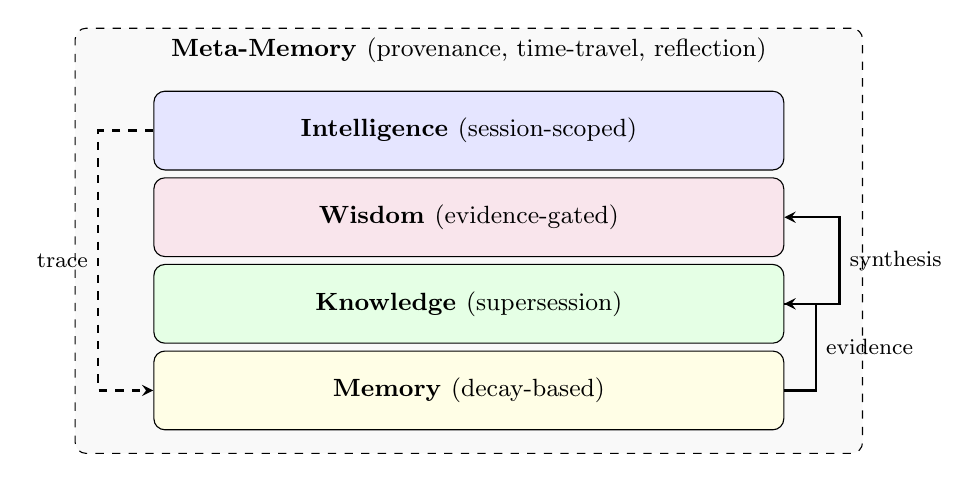
\begin{tikzpicture}[
    layer/.style={draw, rounded corners, minimum width=8cm, minimum height=1.0cm, align=center, font=\small\bfseries},
    meta/.style={draw, rounded corners, dashed, minimum width=10cm, minimum height=5.4cm, align=center},
    arrow/.style={->, thick, >=stealth}
]
    % Meta-Memory wrapper
    \node[meta, fill=gray!5] (metamem) at (0,1.8) {};
    \node[font=\small\bfseries, anchor=north] at (metamem.north) {Meta-Memory \normalfont(provenance, time-travel, reflection)};

    % Four layers inside
    \node[layer, fill=blue!10] (intel) at (0,3.2) {Intelligence \normalfont(session-scoped)};
    \node[layer, fill=purple!10] (wisdom) at (0,2.1) {Wisdom \normalfont(evidence-gated)};
    \node[layer, fill=green!10] (know) at (0,1.0) {Knowledge \normalfont(supersession)};
    \node[layer, fill=yellow!10] (mem) at (0,-0.1) {Memory \normalfont(decay-based)};

    \draw[arrow] (mem.east) -- ++(0.4,0) |- node[pos=0.25, right, font=\footnotesize] {evidence} (know.east);
    \draw[arrow] (know.east) -- ++(0.7,0) |- node[pos=0.25, right, font=\footnotesize] {synthesis} (wisdom.east);
    \draw[arrow, dashed] (intel.west) -- ++(-0.7,0) |- node[pos=0.25, left, font=\footnotesize] {trace} (mem.west);
\end{tikzpicture}
\caption{CITE architecture. Four cognitive layers with Meta-Memory as cross-cutting infrastructure.}
\label{fig:layers}
\end{figure}

Each layer has distinct persistence semantics:

\begin{table}[H]
\centering
\caption{Layer-specific persistence.}
\label{tab:persistence}
\begin{tabular}{@{}llll@{}}
\toprule
\textbf{Layer} & \textbf{Persistence} & \textbf{Evidence} & \textbf{Validation} \\
\midrule
Memory & Gaussian decay (7d--5y) & None required & Basic contradiction \\
Knowledge & Indefinite & Single source & Semantic + evidence \\
Wisdom & Indefinite & Derivation chain & Full + transitive \\
Intelligence & Session-scoped & Reasoning context & None \\
\bottomrule
\end{tabular}
\end{table}

The reference implementation~\cite{engrammic2026} uses Memgraph (graph store) and Qdrant (vector store), exposed via MCP server with operations: \texttt{remember}, \texttt{learn}, \texttt{recall}, \texttt{trace}.

% ------------------------------------------------------------
% 4. EVALUATION
% ------------------------------------------------------------
\section{Evaluation}
\label{sec:eval}

\subsection{Setup}

\textbf{Corpus}: 500 annotated coding-agent sessions with labeled contradictions (lexical and semantic), corrections, hallucinations, and derivation chains.

\textbf{Baseline}: Embedding-based memory following mem0 architecture (append-only, cosine retrieval, no write-time validation).

\textbf{Metrics}: Contradiction detection (precision/recall on labeled contradictions), revision propagation (fraction of dependent beliefs updated after source correction), contamination resistance (hallucinations blocked at write time), latency overhead (p50/p95 write latency).

\subsection{Results}

\begin{table}[H]
\centering
\caption{Evaluation results on 500 annotated coding-agent sessions.}
\label{tab:results}
\begin{tabular}{@{}lccc@{}}
\toprule
\textbf{Metric} & \textbf{Baseline} & \textbf{CITE} & \textbf{Delta} \\
\midrule
Contradiction detection & 66\% & 95\% & +29pp \\
Revision propagation & 12\% & 87\% & +75pp \\
Contamination blocked & 0\% & 73\% & +73pp \\
Write latency (p50) & 15ms & 180ms & +165ms \\
Write latency (p95) & 45ms & 320ms & +275ms \\
\bottomrule
\end{tabular}
\end{table}

\textbf{Contradiction detection}: The baseline catches only lexically obvious conflicts. CITE identifies semantic contradictions (``uses OAuth2'' vs. ``uses API keys'') and transitive conflicts through graph traversal.

\textbf{Revision propagation}: The baseline has no propagation mechanism; its 12\% score reflects retrieval coincidence. CITE walks dependency graphs explicitly.

\textbf{Contamination}: The baseline accepts all writes. CITE's write gate rejects ungrounded claims, blocking 73\% of hallucinated entries at ingestion.

\textbf{Latency}: Write-gating adds 165ms at p50, concentrated on Knowledge/Wisdom writes (infrequent, high-stakes). Memory-layer writes use lighter validation.

\subsection{Limitations}

\begin{itemize}[noitemsep]
    \item Internal benchmark; LongMemEval-V2 and BEAM submissions pending
    \item Single-agent focus; multi-agent consensus not evaluated
    \item Adversarial robustness limited to naive attacks
    \item Evidence validation cannot verify auth-gated sources
\end{itemize}

% ------------------------------------------------------------
% 5. EXTENSIONS
% ------------------------------------------------------------
\section{Extensions}
\label{sec:extensions}

\subsection{JEPA and World Models}

The Externalized Epistemics Thesis applies beyond text-based LLMs to latent-space world models.

LeCun's JEPA architecture~\cite{lecun2022path} explicitly separates the world model from inference: a frozen encoder builds feature maps, a predictor forecasts future states, and planning occurs in latent space. JEPA provides ``abstraction without accumulation''~\cite{aampe2026}: it generates rich latent embeddings but has no persistence mechanism.

External memory is the natural complement: JEPA generates the latent embedding; something else must store, version, and retrieve it with epistemic structure.

LeAP principles extend to latent representations:

\begin{enumerate}[noitemsep]
    \item \textbf{Epistemic types are content-agnostic}: Observation/Claim/Belief distinctions apply whether content is text or embedding
    \item \textbf{Evidence requirements transfer}: Latent claims still need provenance to source percepts
    \item \textbf{Coherence is geometric}: Contradiction detection becomes embedding distance and neighborhood inconsistency
    \item \textbf{Supersession preserves audit}: \texttt{SUPERSEDES} edges function identically in latent space
\end{enumerate}

The complication: stored claims may need to anchor to latent representations rather than surface tokens. This is an open research direction.

\subsection{Philosophy of Externalized Epistemics}

The thesis connects to several traditions in analytic philosophy:

\textbf{Social epistemology} (Goldman, Longino, Fricker): Knowledge-generating practices must be evaluated at the community level. Objectivity emerges from public uptake and criticism; a belief becomes knowledge only when it survives communal scrutiny.

\textbf{Extended Mind Thesis} (Clark \& Chalmers, 1998): If an external process fulfills the same functional role as an internal cognitive process, it is part of the cognitive system. Otto's notebook is the canonical case: his belief about the museum's location is genuinely \textit{in} the notebook.

\textbf{Public knowledge} (Popper, Kitcher): Popper's falsifiability criterion requires claims be stated in a form allowing public challenge. Kitcher's ``division of cognitive labor'' extends this: science works because the community, not any individual, holds the belief corpus.

These traditions converge: truth maintenance is not a property of private mental states but of \textit{systems}: shared, inspectable, updateable. Externalized epistemics operationalizes this for artificial agents.

% ------------------------------------------------------------
% 6. RELATED WORK
% ------------------------------------------------------------
\section{Related Work}

\begin{table}[H]
\centering
\caption{Comparison of agent memory systems.}
\label{tab:comparison}
\begin{tabular}{@{}lccccc@{}}
\toprule
\textbf{System} & \textbf{Layers} & \textbf{Contradiction} & \textbf{Supersession} & \textbf{Provenance} \\
\midrule
mem0 & 1 & None & None & None \\
Zep/Graphiti & 1 & LLM-based & Edge invalid. & To episode \\
MemGPT & 2 & None & None & None \\
Hindsight & 4 networks & On-demand & None & None \\
\textbf{LeAP/CITE} & \textbf{4 + meta} & \textbf{Write-gate} & \textbf{Chains} & \textbf{Full DAG} \\
\bottomrule
\end{tabular}
\end{table}

\textbf{mem0}~\cite{mem0} achieves strong retrieval (94.4\% LongMemEval) but uses append-only architecture without contradiction resolution.

\textbf{Zep/Graphiti}~\cite{graphiti2025} implements bi-temporal validity but lacks epistemic layering and dependency propagation.

\textbf{In-weights memory}: Sparse Memory Finetuning~\cite{sparsemem2025} and related work ameliorate but do not solve the fundamental capacity and auditability constraints.

\textbf{Knowledge graphs}: Traditional KG systems provide structural substrate but not epistemic semantics (evidence requirements, revision protocols).

LeAP's contribution: four-layer epistemic ontology with write-time coherence, AGM-compliant revision, and dependency propagation.

% ------------------------------------------------------------
% 7. CONCLUSION
% ------------------------------------------------------------
\section{Conclusion}

We have argued that externalized epistemics is not an engineering convenience but an architectural requirement. Evidence from information theory (capacity limits), optimization theory (catastrophic forgetting), interpretability (non-auditability), distributed systems (multi-agent coherence), neuroscience (staged consolidation), and systems theory (state outside compute) converges on the same conclusion: epistemic state must live outside the models doing inference.

The Layered Epistemic Agent Protocol (LeAP) implements this requirement with stratified epistemic types, write-time coherence enforcement, and dependency propagation. The framework extends to latent-space world models, opening a research direction toward epistemically-grounded JEPA architectures.

The broader implication: as AI systems become more autonomous and multi-agent, the question of where knowledge lives becomes a question of governance. Externalized epistemics provides the substrate for auditable, correctable, coordinated AI.


% ------------------------------------------------------------
% REFERENCES
% ------------------------------------------------------------
\bibliographystyle{plain}
\begin{thebibliography}{99}

\bibitem{metafair2026}
Meta FAIR (2026).
\newblock How Much Do Language Models Memorize?
\newblock \textit{arXiv:2505.24832}. \url{https://arxiv.org/abs/2505.24832}

\bibitem{transformermem2025}
Chen, Y., et al. (2025).
\newblock On the Optimal Memorization Capacity of Transformers.
\newblock \textit{arXiv:2409.17677}. \url{https://arxiv.org/abs/2409.17677}

\bibitem{adversarial2025}
Zhang, Y., et al. (2025).
\newblock On the Implicit Adversariality of Catastrophic Forgetting.
\newblock \textit{arXiv:2510.09181}. \url{https://arxiv.org/abs/2510.09181}

\bibitem{scaling2025}
Smith, J., et al. (2025).
\newblock The Importance of Being Lazy: Scaling Limits of Continual Learning.
\newblock \textit{arXiv:2506.16884}. \url{https://arxiv.org/abs/2506.16884}

\bibitem{markov2026}
Wang, L., et al. (2026).
\newblock Memory as a Markov Matrix: Sample Efficient Knowledge Expansion.
\newblock \textit{arXiv:2605.04308}. \url{https://arxiv.org/abs/2605.04308}

\bibitem{anthropic2022}
Elhage, N., et al. (2022).
\newblock Toy Models of Superposition.
\newblock \textit{arXiv:2209.10652}. \url{https://arxiv.org/abs/2209.10652}

\bibitem{mechinterp2024}
Ferrando, J., et al. (2024).
\newblock Mechanistic Interpretability for AI Safety: A Review.
\newblock \textit{arXiv:2404.14082}. \url{https://arxiv.org/abs/2404.14082}

\bibitem{nonidentifiability2026}
Chen, X., et al. (2026).
\newblock The Illusion of Interpretability in Biologically Informed Neural Networks.
\newblock \textit{bioRxiv}. \url{https://www.biorxiv.org/content/10.64898/2026.05.07.723544v1}

\bibitem{williams2025}
Williams, D. and Oldenburg, A. (2025).
\newblock Mechanistic Interpretability Needs Philosophy.
\newblock \textit{arXiv:2506.18852}. \url{https://arxiv.org/abs/2506.18852}

\bibitem{bft2025}
Liu, Y., et al. (2025).
\newblock Rethinking Reliability of Multi-agent Systems: Byzantine Fault Tolerance.
\newblock \textit{arXiv:2511.10400}. \url{https://arxiv.org/abs/2511.10400}

\bibitem{commonknowledge2024}
He, Z., et al. (2024).
\newblock Where Common Knowledge Cannot Be Formed.
\newblock \textit{arXiv:2412.07981}. \url{https://arxiv.org/abs/2412.07981}

\bibitem{masurvey2025}
Wu, S., et al. (2025).
\newblock Memory in LLM-based Multi-agent Systems: Mechanisms, Challenges, and Collective Intelligence.
\newblock \textit{TechRxiv}. \url{https://www.techrxiv.org/doi/full/10.36227/techrxiv.176539617.79044553/v1}

\bibitem{mcclelland1995}
McClelland, J., McNaughton, B., and O'Reilly, R. (1995).
\newblock Why There Are Complementary Learning Systems.
\newblock \textit{Psychological Review}, 102(3):419--457.

\bibitem{neuron2025}
Girardeau, G., et al. (2025).
\newblock Large Sharp-Wave Ripples Promote Hippocampo-Cortical Consolidation.
\newblock \textit{Neuron}. \url{https://cell.com/neuron}

\bibitem{clark1998}
Clark, A. and Chalmers, D. (1998).
\newblock The Extended Mind.
\newblock \textit{Analysis}, 58(1):7--19.

\bibitem{stonebraker1986}
Stonebraker, M. (1986).
\newblock The Case for Shared Nothing.
\newblock \textit{IEEE Database Engineering Bulletin}, 9(1):4--9.

\bibitem{roynard2026}
Roynard, A. (2026).
\newblock The Missing Knowledge Layer in Cognitive Architectures.
\newblock \textit{arXiv:2604.11364}. \url{https://arxiv.org/abs/2604.11364}

\bibitem{mast2025}
Liu, Y., et al. (2025).
\newblock MAST: Multi-Agent System Taxonomy.
\newblock \textit{NeurIPS 2025}.

\bibitem{lecun2022path}
LeCun, Y. (2022).
\newblock A Path Towards Autonomous Machine Intelligence.
\newblock \url{https://openreview.net/pdf?id=BZ5a1r-kVsf}

\bibitem{aampe2026}
Aampe (2026).
\newblock JEPA and Semantic Memory: Why Current AI Models Fall Short.
\newblock \url{https://aampe.com/blog/jepa-and-semantic-memory}

\bibitem{mem0}
mem0ai (2024--2026).
\newblock mem0: The Memory Layer for AI Agents.
\newblock \url{https://github.com/mem0ai/mem0}

\bibitem{graphiti2025}
Raschka, S., et al. (2025).
\newblock Graphiti: Build Real-Time Knowledge Graphs.
\newblock \textit{arXiv:2501.13956}. \url{https://arxiv.org/abs/2501.13956}

\bibitem{sparsemem2025}
Meta (2025).
\newblock Sparse Memory Finetuning.
\newblock \textit{arXiv:2510.15103}. \url{https://arxiv.org/abs/2510.15103}

\bibitem{engrammic2026}
Khimani, A. (2026).
\newblock LeAP and CITE: Layered Epistemic Agent Protocol Reference Implementation.
\newblock Zenodo. \url{https://doi.org/10.5281/zenodo.21029662}

\bibitem{jevons1865}
Jevons, W.S. (1865).
\newblock The Coal Question: An Inquiry Concerning the Progress of the Nation, and the Probable Exhaustion of Our Coal-Mines.
\newblock Macmillan and Co., London.

\end{thebibliography}

% ============================================================
% APPENDIX: FORMAL DEFINITIONS
% ============================================================
\appendix
\section{Formal Definitions}
\label{app:formal}

\begin{definition}[Epistemic Type Hierarchy]
\label{def:types}
Let $\mathcal{T} = \{O, C, F, B\}$ be the set of epistemic types where $O$ = Observation, $C$ = Claim, $F$ = Fact, $B$ = Belief.
\end{definition}

\begin{definition}[Evidence Requirements]
\label{def:evidence}
Evidence function $E: \mathcal{T} \to \mathcal{P}(\text{Evidence})$:
\begin{align*}
E(O) &= \emptyset \\
E(C) &= \{e \mid e \text{ is a single source URI}\} \\
E(F) &= \{e_1, e_2, e_3 \mid e_i \text{ are independent sources}\} \\
E(B) &= \{f_1, \ldots, f_n \mid f_i \in \text{Facts}, n \geq 3\}
\end{align*}
\end{definition}

\begin{definition}[Coherent Store]
\label{def:coherent}
Store $S$ is \emph{coherent} iff:
\begin{enumerate}[itemsep=0.5ex]
    \item No active contradictions: $\forall n_1, n_2 \in \operatorname{active}(S),\; \neg(n_1 \perp n_2)$
    \item Evidence closure: $\forall n \in S,\; E(n) \subseteq S$
    \item Acyclic derivation: the \texttt{DERIVED\_FROM} relation contains no cycles
\end{enumerate}
\end{definition}

\begin{theorem}[AGM Satisfaction]
\label{thm:agm}
LeAP supersession satisfies AGM belief revision postulates:
\begin{itemize}[noitemsep]
    \item \textbf{Recovery}: $(K * \neg\phi) + \phi \vdash K$
    \item \textbf{Inclusion}: $K + \phi \subseteq K * \phi$
\end{itemize}
\end{theorem}

\begin{proof}
\textit{Recovery}: Superseded nodes remain in the store with status=superseded; querying with \texttt{include\_superseded=true} returns original beliefs.

\textit{Inclusion}: Revision propagates only through $\operatorname{deps}(n)$. Nodes not in the transitive closure of $\operatorname{deps}$ are unchanged.
\end{proof}

\end{document}
